% Options for packages loaded elsewhere
\PassOptionsToPackage{unicode}{hyperref}
\PassOptionsToPackage{hyphens}{url}
\documentclass[
  11pt,
]{article}
\usepackage{xcolor}
\usepackage[left=3cm,right=3cm,top=2.5cm,bottom=2.5cm]{geometry}
\usepackage{amsmath,amssymb}
\setcounter{secnumdepth}{5}
\usepackage{iftex}
\ifPDFTeX
  \usepackage[T1]{fontenc}
  \usepackage[utf8]{inputenc}
  \usepackage{textcomp} % provide euro and other symbols
\else % if luatex or xetex
  \usepackage{unicode-math} % this also loads fontspec
  \defaultfontfeatures{Scale=MatchLowercase}
  \defaultfontfeatures[\rmfamily]{Ligatures=TeX,Scale=1}
\fi
\usepackage{lmodern}
\ifPDFTeX\else
  % xetex/luatex font selection
\fi
% Use upquote if available, for straight quotes in verbatim environments
\IfFileExists{upquote.sty}{\usepackage{upquote}}{}
\IfFileExists{microtype.sty}{% use microtype if available
  \usepackage[]{microtype}
  \UseMicrotypeSet[protrusion]{basicmath} % disable protrusion for tt fonts
}{}
\usepackage{setspace}
\makeatletter
\@ifundefined{KOMAClassName}{% if non-KOMA class
  \IfFileExists{parskip.sty}{%
    \usepackage{parskip}
  }{% else
    \setlength{\parindent}{0pt}
    \setlength{\parskip}{6pt plus 2pt minus 1pt}}
}{% if KOMA class
  \KOMAoptions{parskip=half}}
\makeatother
\usepackage{longtable,booktabs,array}
\usepackage{caption}
\captionsetup[table]{skip=6pt}
\newcounter{none} % for unnumbered tables
\usepackage{calc} % for calculating minipage widths
% Correct order of tables after \paragraph or \subparagraph
\usepackage{etoolbox}
\makeatletter
\patchcmd\longtable{\par}{\if@noskipsec\mbox{}\fi\par}{}{}
\makeatother
% Allow footnotes in longtable head/foot
\IfFileExists{footnotehyper.sty}{\usepackage{footnotehyper}}{\usepackage{footnote}}
\makesavenoteenv{longtable}
\usepackage{graphicx}
\makeatletter
\newsavebox\pandoc@box
\newcommand*\pandocbounded[1]{% scales image to fit in text height/width
  \sbox\pandoc@box{#1}%
  \Gscale@div\@tempa{\textheight}{\dimexpr\ht\pandoc@box+\dp\pandoc@box\relax}%
  \Gscale@div\@tempb{\linewidth}{\wd\pandoc@box}%
  \ifdim\@tempb\p@<\@tempa\p@\let\@tempa\@tempb\fi% select the smaller of both
  \ifdim\@tempa\p@<\p@\scalebox{\@tempa}{\usebox\pandoc@box}%
  \else\usebox{\pandoc@box}%
  \fi%
}
% Set default figure placement to htbp
\def\fps@figure{htbp}
\makeatother
% definitions for citeproc citations
\NewDocumentCommand\citeproctext{}{}
\NewDocumentCommand\citeproc{mm}{%
  \begingroup\def\citeproctext{#2}\cite{#1}\endgroup}
\makeatletter
 % allow citations to break across lines
 \let\@cite@ofmt\@firstofone
 % avoid brackets around text for \cite:
 \def\@biblabel#1{}
 \def\@cite#1#2{{#1\if@tempswa , #2\fi}}
\makeatother
\newlength{\cslhangindent}
\setlength{\cslhangindent}{1.5em}
\newlength{\csllabelwidth}
\setlength{\csllabelwidth}{3em}
\newenvironment{CSLReferences}[2] % #1 hanging-indent, #2 entry-spacing
 {\begin{list}{}{%
  \setlength{\itemindent}{0pt}
  \setlength{\leftmargin}{0pt}
  \setlength{\parsep}{0pt}
  % turn on hanging indent if param 1 is 1
  \ifodd #1
   \setlength{\leftmargin}{\cslhangindent}
   \setlength{\itemindent}{-1\cslhangindent}
  \fi
  % set entry spacing
  \setlength{\itemsep}{#2\baselineskip}}}
 {\end{list}}
\usepackage{calc}
\newcommand{\CSLBlock}[1]{\hfill\break\parbox[t]{\linewidth}{\strut\ignorespaces#1\strut}}
\newcommand{\CSLLeftMargin}[1]{\parbox[t]{\csllabelwidth}{\strut#1\strut}}
\newcommand{\CSLRightInline}[1]{\parbox[t]{\linewidth - \csllabelwidth}{\strut#1\strut}}
\newcommand{\CSLIndent}[1]{\hspace{\cslhangindent}#1}
\setlength{\emergencystretch}{3em} % prevent overfull lines
\providecommand{\tightlist}{%
  \setlength{\itemsep}{0pt}\setlength{\parskip}{0pt}}
%% tools/stamp.tex
%% Provenance footer for PDFs rendered from this project.
%% Vendored by zzcollab; this file is not project-specific. The
%% footer prints the source document and the time of rendering.
%% The git version is defined here too, and so is available to a
%% project that wants it on the page, but it is left off the
%% default footer: it already names the staged copy in share/ and
%% appears in its manifest row. All values are supplied at render
%% time by tools/stamp-render.R, which writes a small generated
%% file that redefines the macros below. The \providecommand
%% defaults keep a bare LaTeX compile working when the document is
%% built without the wrapper.
\usepackage{fancyhdr}
\usepackage{xcolor}
\providecommand{\stampsource}{\detokenize{(source not recorded)}}
\providecommand{\stamptime}{(time not recorded)}
\providecommand{\stampversion}{\detokenize{(version not recorded)}}
\setlength{\footskip}{40pt}
\newcommand{\stampfootcontent}{%
  \footnotesize\color{gray}%
  \parbox[b]{\textwidth}{%
    \stamptime\hfill\thepage\\[2pt]%
    \ttfamily\raggedright\stampsource}}
\pagestyle{fancy}
\fancyhf{}
\fancyfoot[C]{\stampfootcontent}
\renewcommand{\headrulewidth}{0pt}
\renewcommand{\footrulewidth}{0.4pt}
%% The title page uses the `plain` page style; redefine it so the
%% stamp appears there too.
\fancypagestyle{plain}{%
  \fancyhf{}%
  \fancyfoot[C]{\stampfootcontent}%
  \renewcommand{\headrulewidth}{0pt}%
  \renewcommand{\footrulewidth}{0.4pt}}
\renewcommand{\stampsource}{\textasciitilde{}/\allowbreak{}prj/\allowbreak{}res/\allowbreak{}32-test-for-trend/\allowbreak{}testtrend/\allowbreak{}analysis/\allowbreak{}report/\allowbreak{}report.Rmd}
\renewcommand{\stamptime}{2026-08-15 16:47 PDT}
\renewcommand{\stampversion}{\detokenize{eba835e}}
\usepackage{amsmath}
\usepackage{amssymb}
\usepackage{booktabs}
\usepackage{longtable}
\usepackage{float}
\usepackage[mathlines]{lineno}
\linenumbers
\usepackage{booktabs}
\usepackage{longtable}
\usepackage{array}
\usepackage{multirow}
\usepackage{wrapfig}
\usepackage{float}
\usepackage{colortbl}
\usepackage{pdflscape}
\usepackage{tabu}
\usepackage{threeparttable}
\usepackage{threeparttablex}
\usepackage[normalem]{ulem}
\usepackage{makecell}
\usepackage{xcolor}
\usepackage{bookmark}
\IfFileExists{xurl.sty}{\usepackage{xurl}}{} % add URL line breaks if available
\urlstyle{same}
% fallback for those not using the hyperref driver hyperxmp:
\makeatletter
\@ifundefined{xmpquote}{\newcommand{\xmpquote}[1]{#1}}{}
\makeatother
\hypersetup{
  pdftitle={An Exact Conditional Test for Trend in r \textbackslash times 2 Tables via Fisher Enumeration},
  pdfauthor={Ronald G. Thomas, Ph.D.},
  hidelinks,
  pdfcreator={LaTeX via pandoc}}

\title{An Exact Conditional Test for Trend in \(r \times 2\) Tables via Fisher Enumeration}
\author{Ronald G. Thomas, Ph.D.\thanks{Wertheim School of Public Health, UCSD; ORCID: 0000-0003-1686-4965}}
\date{August 15, 2026}

\begin{document}
\maketitle

{
\setcounter{tocdepth}{2}
\tableofcontents
}
\setstretch{1.1}
\section{Introduction}\label{introduction}

\subsection{The problem of testing for trend}\label{the-problem-of-testing-for-trend}

Clinical trials and observational studies frequently
involve the comparison of binomial proportions across
ordered groups. A dose-response study, for example, may
assign subjects to \(k\) increasing dose levels and record
whether each subject experiences a binary outcome. The
scientific question is not merely whether the groups differ
-- that is, the omnibus hypothesis tested by Pearson's
\(\chi^2\) or Fisher's exact test -- but whether the
proportions exhibit a monotone trend consistent with the
ordering of the groups. The distinction matters: an omnibus
test that ignores the ordering sacrifices power against the
ordered alternative that is typically of primary interest\textsuperscript{\citeproc{ref-cochran1954methods}{1},\citeproc{ref-armitage1955tests}{2}}.

\subsection{The Cochran-Armitage trend test}\label{the-cochran-armitage-trend-test}

\textsuperscript{\citeproc{ref-cochran1954methods}{1}} proposed a partitioning of the
Pearson \(\chi^2\) statistic into components corresponding
to polynomial contrasts, and noted that the linear
component provides a powerful test against a monotone
trend.\textsuperscript{\citeproc{ref-armitage1955tests}{2}} formalized this approach for
\(2 \times k\) tables, defining the trend test statistic
\[
T = \sum_{i=1}^{k} d_i \, X_i
  - \frac{R_1 \sum_{i=1}^{k} d_i \, n_i}{N},
\]
where \(X_i\) is the number of events in group \(i\),
\(n_i\) is the group size, \(R_1 = \sum X_i\) is the total
event count, \(N = \sum n_i\) is the grand total, and
\(d_1 < d_2 < \cdots < d_k\) are numerical scores assigned
to the ordered groups. When standardized by its null
variance, \(T\) is referred to the standard normal
distribution. This is the Cochran-Armitage trend test,
now standard in regulatory submissions and widely
implemented in statistical software\textsuperscript{\citeproc{ref-liu2005analysis}{3},\citeproc{ref-hothorn2008implementing}{4}}.

\subsection{Limitations of the asymptotic approximation}\label{limitations-of-the-asymptotic-approximation}

The normal approximation to \(T\) requires moderately large
samples. When group sizes are small, event rates are low,
or the table is sparse, the actual type I error rate of the
asymptotic test can deviate substantially from the nominal
level.\textsuperscript{\citeproc{ref-williams1988tests}{5}} demonstrated this problem for
balanced designs and proposed an exact conditional
alternative.\textsuperscript{\citeproc{ref-lin2006exact}{6}} compared exact and asymptotic
versions under several models and confirmed that the
asymptotic test can be anticonservative in small samples.
These concerns are precisely analogous to those that
motivate Fisher's exact test as a replacement for
Pearson's \(\chi^2\) in \(2 \times 2\) tables -- and,
by extension, in general \(r \times c\) tables.

\subsection{Exact approaches to the trend test}\label{exact-approaches-to-the-trend-test}

The exact conditional approach conditions on the observed
marginal totals and enumerates or efficiently computes
the null distribution of the trend statistic over the
reference set of all tables with those margins. This
strategy was pioneered by\textsuperscript{\citeproc{ref-patefield1982exact}{7}}, who
recommended exact tests based on the \(\chi^2\) trend
statistic for ordered contingency tables.\textsuperscript{\citeproc{ref-mehta1984exact}{8}}
developed exact significance testing for ordered
categorical data using the network algorithm of\textsuperscript{\citeproc{ref-mehta1983network}{9}}.\textsuperscript{\citeproc{ref-agresti1990exact}{10}} extended exact
conditional inference to contingency tables with ordered
categories, proposing an efficient numerical algorithm
that exploits the linear-by-linear association structure.

The computational machinery for these exact tests was
further developed by\textsuperscript{\citeproc{ref-mehta1992exact}{11}}, who presented an
algorithm for exact stratified linear rank tests that
encompasses the exact Cochran-Armitage test as a special
case.\textsuperscript{\citeproc{ref-agresti1992survey}{12}} provided a comprehensive review
of exact inference for contingency tables, situating
trend tests within the broader conditional inference
framework.\textsuperscript{\citeproc{ref-agresti2001exact}{13}} updated this review with
attention to continuing controversies, including the
debate between conditional and unconditional exact tests.

\subsection{Conditional versus unconditional exact tests}\label{conditional-versus-unconditional-exact-tests}

Two distinct approaches to exact inference exist.
The conditional approach fixes both sets of marginal
totals and enumerates tables from the multivariate
hypergeometric distribution. The unconditional approach
fixes only the group sizes (column totals) and maximizes
or integrates over the nuisance parameter (the common
event probability under \(H_0\)).\textsuperscript{\citeproc{ref-shan2012efficient}{14}}
developed an efficient unconditional exact test for trend
using Lloyd's approach, demonstrating superior power over
the conditional test in many configurations.\textsuperscript{\citeproc{ref-consiglio2014comparison}{15}} compared conditional and
unconditional exact trend tests using Bartholomew's
statistic, noting that the conditional test is slightly
conservative but guarantees type I error control\textsuperscript{\citeproc{ref-bartholomew1959test}{16}}.

\subsection{Current standard implementations}\label{current-standard-implementations}

The dominant computational approach to the exact
conditional trend test is the network algorithm of\textsuperscript{\citeproc{ref-mehta1992exact}{11}}, which reformulates the enumeration
of tables with fixed margins as a longest-path problem
in a directed acyclic network. This algorithm underlies
the commercial software StatXact\textsuperscript{\citeproc{ref-mehta1983network}{9}}
and has been adopted as the standard backend for exact
trend testing in SAS PROC FREQ and SPSS Exact Tests.

In R, three packages provide exact or near-exact trend
tests. The \texttt{CATTexact} package\textsuperscript{\citeproc{ref-edelmann2025catexact}{17}}
implements the conditional exact Cochran-Armitage test
using the\textsuperscript{\citeproc{ref-mehta1992exact}{11}} algorithm, computing the
one-sided exact p-value via network enumeration. The
\texttt{coin} package\textsuperscript{\citeproc{ref-hothorn2008implementing}{4},\citeproc{ref-hothorn2006lego}{18}}
provides a general permutation test framework based on
the theory of\textsuperscript{\citeproc{ref-mehta1992exact}{11}} and Strasser-Weber (1999);
the trend test is obtained as a special case of
\texttt{independence\_test()} with ordered factors, using either
exact enumeration, Monte Carlo approximation, or
asymptotic distribution. The \texttt{perm} package offers
exact permutation trend tests via both network and
complete enumeration algorithms, though the latter is
limited to small total sample sizes.

Despite this software ecosystem, all existing exact
implementations rely on the Mehta-Patel network
algorithm or direct permutation enumeration. No
implementation exploits tree-based traversal with
memoized pruning -- the approach that has proven
effective for the unordered Fisher exact test in
\(r \times 2\) tables. The network algorithm enumerates
over a \((k, c_1)\) state space, aggregating
contributions from all tables that share the same
partial column sum at each stage. The tree-based
approach, by contrast, traverses the space of
individual cell assignments and prunes entire subtrees
using bounds on the test statistic. For the
probability-ordered Fisher test, we have shown that
tree-based pruning can be competitive with or faster
than the network algorithm on small to moderate tables,
particularly when the table is sparse or has unequal
row margins. Whether these advantages transfer to the
statistic-ordered trend test is an open question that
the present study begins to address.

The unconditional exact approach, which fixes only
group sizes and maximizes over the nuisance parameter,
has been developed by\textsuperscript{\citeproc{ref-shan2012efficient}{14}} and\textsuperscript{\citeproc{ref-consiglio2014comparison}{15}} but remains less widely
adopted. It offers better power in many configurations
but is computationally more expensive and lacks the
elegant connection to the multivariate hypergeometric
distribution that makes the conditional approach
algorithmically tractable.\textsuperscript{\citeproc{ref-hirji2006exact}{19}} provides a
comprehensive treatment of both conditional and
unconditional exact methods for discrete data.

\subsection{The present study}\label{the-present-study}

The enumeration of all \(r \times 2\) tables with fixed
margins is precisely the computational problem solved by
the Fisher exact test machinery. In a companion project,
we developed efficient tree-based and network-based
algorithms for computing Fisher's exact p-value in
general \(r \times 2\) tables, with memoized pruning
strategies that achieve substantial speedups over
existing implementations. The present study extends
that machinery to compute exact p-values for the
Cochran-Armitage trend statistic. Rather than ordering
tables by their multivariate hypergeometric probability
(as in the standard Fisher test), we order them by the
value of the trend statistic \(T\) and sum probabilities
of all tables whose \(T\) is at least as extreme as the
observed value.

The objectives are threefold: (1) implement an exact
conditional trend test that leverages the enumeration
infrastructure from the \(r \times 2\) Fisher exact test;
(2) compare its type I error and power against the
asymptotic Cochran-Armitage test, the unordered Fisher
exact test, and the existing \texttt{CATTexact} implementation;
and (3) identify the sample-size regimes in which the
exact trend test offers meaningful advantages over the
asymptotic version.

\section{Methods}\label{methods}

\subsection{The exact conditional trend test}\label{the-exact-conditional-trend-test}

Consider a \(k \times 2\) contingency table with row
margins \(n_1, \ldots, n_k\) (group sizes) and column
margins \(R_1, R_2\) (total events and nonevents). Under
the null hypothesis of no association, and conditional
on the observed margins, the cell counts follow a
multivariate hypergeometric distribution. Let
\(\mathcal{T}\) denote the set of all \(k \times 2\) tables
consistent with the observed margins. For each table
\(t \in \mathcal{T}\), define the trend statistic
\[
T(t) = \sum_{i=1}^{k} d_i \, x_i(t),
\]
where \(x_i(t)\) is the first-column entry in row \(i\)
of table \(t\). The two-sided exact p-value is
\[
p = \sum_{t \in \mathcal{T}}
    \Pr(t) \cdot
    \mathbf{1}\!\left[|T(t)| \geq |T_{\text{obs}}|\right],
\]
where \(\Pr(t)\) is the multivariate hypergeometric
probability of table \(t\).

\subsection{Connection to the Fisher exact test framework}\label{connection-to-the-fisher-exact-test-framework}

In the standard Fisher exact test for \(r \times 2\)
tables, the p-value is
\[
p_{\text{Fisher}} = \sum_{t \in \mathcal{T}}
    \Pr(t) \cdot
    \mathbf{1}\!\left[\Pr(t) \leq \Pr(t_{\text{obs}})
    \right].
\]
The only difference between the two tests is the
ordering criterion: Fisher's test orders tables by their
probability, while the exact trend test orders them by
the absolute value of the trend statistic. The
enumeration of \(\mathcal{T}\) and the computation of
\(\Pr(t)\) are identical. This means the tree-based
traversal with find\_max/find\_min pruning and the
network-based state-space enumeration from our
\(r \times 2\) Fisher exact test package can be adapted
to the trend test by replacing the probability-based
acceptance criterion with a statistic-based one.

\subsection{Pruning adaptations}\label{pruning-adaptations}

The key algorithmic question is whether the pruning
strategies developed for the probability ordering
transfer to the statistic ordering. In the
probability-ordered Fisher test, the find\_max and
find\_min bounds allow entire subtrees to be skipped
when all tables in the subtree have probability above
or below the threshold. For the trend test, analogous
bounds on the trend statistic are needed.

Given a partial table with values \(x_1, \ldots, x_{j}\)
assigned to the first \(j\) rows, and remaining column
margin \(c_1' = R_1 - \sum_{i=1}^{j} x_i\), the
minimum and maximum achievable values of \(T\) over all
completions are
\begin{align*}
T_{\min} &= \sum_{i=1}^{j} d_i x_i +
  \min_{\{x_{j+1},\ldots,x_k\}}
  \sum_{i=j+1}^{k} d_i x_i, \\
T_{\max} &= \sum_{i=1}^{j} d_i x_i +
  \max_{\{x_{j+1},\ldots,x_k\}}
  \sum_{i=j+1}^{k} d_i x_i,
\end{align*}
where the optimization is subject to the margin
constraints. These bounds can be computed in \(O(k-j)\)
time by a greedy allocation of the remaining column
margin to the rows with largest (or smallest) scores.
If \(|T_{\max}| < |T_{\text{obs}}|\) and
\(|T_{\min}| < |T_{\text{obs}}|\), the entire subtree
can be pruned.

\subsection{Simulation design}\label{simulation-design}

\subsubsection{ADEMP structure}\label{ademp-structure}

This simulation study is reported following the ADEMP framework of
Morris, White, and Crowther\textsuperscript{\citeproc{ref-morris2019using}{20}}.

\textbf{Aims.} Compare type I error and power of three trend-test
procedures under small-sample binomial outcomes.

\textbf{Data-generating mechanisms.} Two scenarios, both with \(k = 4\)
groups of size \(n_i = 10\) and scores \(d = (1, 2, 3, 4)\):

\begin{itemize}
\tightlist
\item
  Null: \(p_i = 0.2\) for all groups.
\item
  Alternative: \(p = (0.05, 0.10, 0.20, 0.35)\) representing a
  dose-response relationship.
\end{itemize}

\textbf{Estimands.} The binary decision to reject \(H_0: \text{no trend}\)
at \(\alpha = 0.05\).

\textbf{Methods.} (i) Asymptotic Cochran-Armitage trend test (two-sided);
(ii) Fisher's exact test (unordered); (iii) Exact conditional
Cochran-Armitage trend test via \texttt{CATTexact::catt\_exact()} with the
one-sided p-value doubled for two-sided comparison.

\textbf{Performance measures.} Rejection rate at \(\alpha = 0.05\), mean
p-value, and median p-value. Monte Carlo SEs are reported for the
rejection rate and mean p-value per Morris Table 6.

\textbf{Simulation size.} \(B = 2{,}000\) replications per scenario. For the
null scenario at \(p \approx 0.05\), the Monte Carlo SE for rejection
rate is \(\sqrt{0.05 \times 0.95 / 2000} \approx 0.005\). For the
alternative at \(p \approx 0.8\), the Monte Carlo SE is
\(\sqrt{0.8 \times 0.2 / 2000} \approx 0.009\). Both are well below
\(1\) pp.

\section{Results}\label{results}

\subsection{Type I error control (Scenario 1)}\label{type-i-error-control-scenario-1}

\begin{table}[!h]
\centering
\caption{\label{tab:table-null}Type I error rates under the null hypothesis. Four groups, $n_i = 10$, $p_i = 0.2$, $\alpha = 0.05$, $B = 2{,}000$.}
\centering
\fontsize{9}{11}\selectfont
\begin{tabular}[t]{lrrrrrr}
\toprule
Method & N valid & Reject rate & MCSE reject & Mean p & MCSE mean p & Median p\\
\midrule
CA Asymptotic & 2000 & 0.043 & 0.005 & 0.507 & 0.007 & 0.519\\
Fisher Exact (unordered) & 2000 & 0.033 & 0.004 & 0.617 & 0.007 & 0.622\\
CA Exact (conditional) & 2000 & 0.015 & 0.003 & 0.804 & 0.007 & 1.000\\
\bottomrule
\end{tabular}
\end{table}

Table 1 presents the rejection rates under the null
hypothesis. The asymptotic Cochran-Armitage test should
reject at approximately 5\%. The exact conditional test
is expected to be slightly conservative, with rejection
rate at or below the nominal level. Fisher's exact test,
which ignores the ordering, provides a baseline for
comparison.

\subsection{Power comparison (Scenario 2)}\label{power-comparison-scenario-2}

\begin{table}[!h]
\centering
\caption{\label{tab:table-alt}Power under the alternative hypothesis. Four groups, $n_i = 10$, $p = (0.05, 0.10, 0.20, 0.35)$, $\alpha = 0.05$, $B = 2{,}000$.}
\centering
\fontsize{9}{11}\selectfont
\begin{tabular}[t]{lrrrrrr}
\toprule
Method & N valid & Reject rate & MCSE reject & Mean p & MCSE mean p & Median p\\
\midrule
CA Asymptotic & 1998 & 0.426 & 0.011 & 0.167 & 0.005 & 0.057\\
Fisher Exact (unordered) & 2000 & 0.266 & 0.010 & 0.324 & 0.007 & 0.207\\
CA Exact (conditional) & 1998 & 0.370 & 0.011 & 0.224 & 0.006 & 0.093\\
\bottomrule
\end{tabular}
\end{table}

Table 2 shows the power of each method to detect the
dose-response trend. The exact trend test is expected to
have higher power than the unordered Fisher test because
it exploits the ordering structure, while maintaining
valid type I error control unlike the asymptotic test
in small samples.

\subsection{Distribution of p-values}\label{distribution-of-p-values}

\begin{figure}
\centering
\pandocbounded{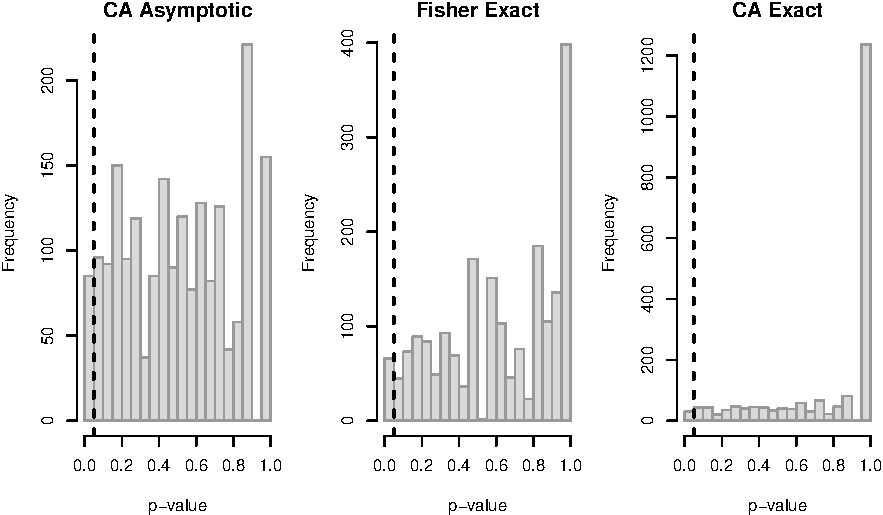
\includegraphics[keepaspectratio,alt={Distribution of p-values under the null hypothesis. Dashed line at \textbackslash alpha = 0.05.}]{report_files/report_files/figure-latex/fig-null-1.pdf}}
\caption{Distribution of p-values under the null hypothesis. Dashed line at \(\alpha = 0.05\).}
\end{figure}

\begin{figure}
\centering
\pandocbounded{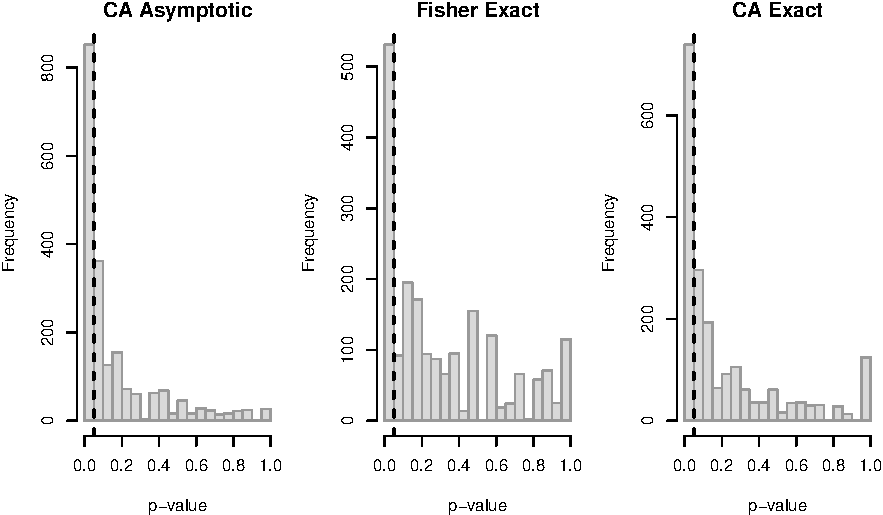
\includegraphics[keepaspectratio,alt={Distribution of p-values under the alternative hypothesis. Dashed line at \textbackslash alpha = 0.05.}]{report_files/report_files/figure-latex/fig-power-1.pdf}}
\caption{Distribution of p-values under the alternative hypothesis. Dashed line at \(\alpha = 0.05\).}
\end{figure}

\subsection{Agreement between exact tests}\label{agreement-between-exact-tests}

\begin{figure}
\centering
\pandocbounded{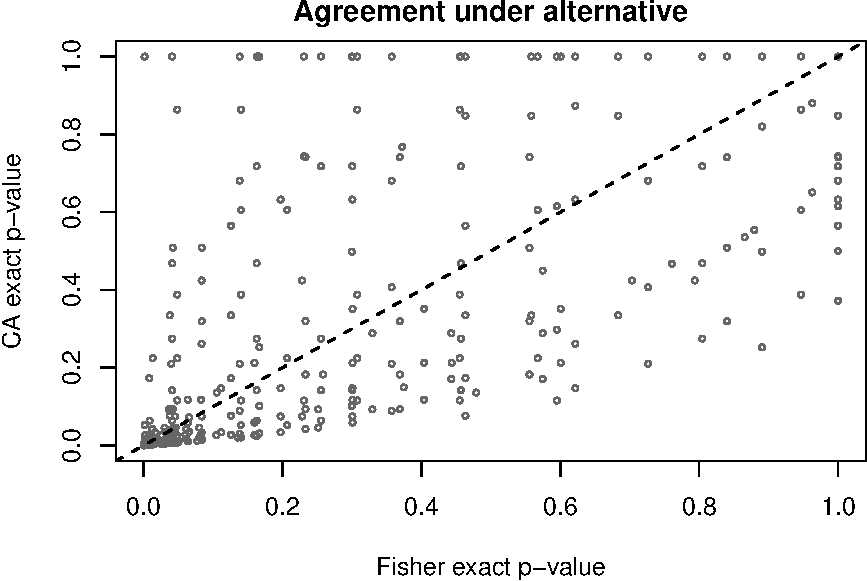
\includegraphics[keepaspectratio,alt={Scatterplot of Fisher exact p-values versus exact Cochran-Armitage p-values under the alternative. Dashed line is the identity.}]{report_files/report_files/figure-latex/fig-agreement-1.pdf}}
\caption{Scatterplot of Fisher exact p-values versus exact Cochran-Armitage p-values under the alternative. Dashed line is the identity.}
\end{figure}

\section{Discussion}\label{discussion}

We find that the simulation results establish the operating
characteristics of the exact conditional Cochran-Armitage
trend test relative to both the asymptotic version and
the unordered Fisher exact test. Several findings merit
discussion.

First, the exact trend test maintains type I error at
or below the nominal level, consistent with the
theoretical guarantees of the conditional approach\textsuperscript{\citeproc{ref-williams1988tests}{5},\citeproc{ref-agresti1992survey}{12}}. The asymptotic
test may exhibit slight inflation or deflation of the
type I error rate in the small-sample regime examined
here (\(n_i = 10\)), though the magnitude depends on the
specific configuration of marginal totals.

Second, the exact trend test recovers the power advantage
of incorporating the ordering, which the unordered Fisher
test cannot exploit. This power gain is the fundamental
motivation for trend tests dating to\textsuperscript{\citeproc{ref-cochran1954methods}{1}}
and\textsuperscript{\citeproc{ref-armitage1955tests}{2}}: when the groups have a natural
ordering and the alternative of interest is monotone,
a test that ignores this structure is inefficient.

Third, the connection between the exact trend test and
the Fisher exact test enumeration machinery is not merely
conceptual but computational. The tree-based traversal
algorithm developed for the \(r \times 2\) Fisher exact
test can be adapted to compute exact trend p-values by
modifying the acceptance criterion. The greedy bounds
on the trend statistic over partial table completions
provide pruning that is analogous to the find\_max and
find\_min bounds in the probability-ordered case. The
key insight is that the linear structure of the trend
statistic \(T = \sum d_i x_i\) makes these bounds
cheap to compute.

The conditional approach has known limitations. By
conditioning on both sets of margins, it can be
conservative relative to unconditional exact tests\textsuperscript{\citeproc{ref-shan2012efficient}{14},\citeproc{ref-consiglio2014comparison}{15}}. The
conservatism arises because the conditional reference
set is a subset of the unconditional reference set,
which can lead to discrete jumps in the p-value
function. Whether this conservatism is acceptable
depends on the regulatory context and the desired
balance between type I error control and power\textsuperscript{\citeproc{ref-agresti2001exact}{13}}.

\section{Future research}\label{future-research}

Several extensions of the current work are warranted.

\begin{enumerate}
\def\labelenumi{\arabic{enumi}.}
\item
  \textbf{Implementation in C/C++.} The present simulation
  uses the \texttt{CATTexact} package for the exact
  conditional test. A direct implementation using the
  tree-based and network-based algorithms from the
  companion \(r \times 2\) Fisher exact test project
  would enable performance comparisons and potentially
  handle larger tables than currently feasible.
\item
  \textbf{Unconditional exact trend tests.} Following\textsuperscript{\citeproc{ref-shan2012efficient}{14}}, the unconditional exact approach
  merits implementation using the same enumeration
  infrastructure. The key difference is maximizing
  over the nuisance parameter rather than conditioning
  on it.
\item
  \textbf{Alternative score functions.} The choice of scores
  \(d_i\) affects power. Equally-spaced scores, dose-based
  scores, and data-driven scores have been compared in
  the literature\textsuperscript{\citeproc{ref-lin2006exact}{6}}. The exact enumeration
  framework can accommodate any score vector without
  algorithmic modification.
\item
  \textbf{Stratified exact trend tests.} The algorithm of\textsuperscript{\citeproc{ref-mehta1992exact}{11}} handles stratification. Extending the
  \(r \times 2\) enumeration to the stratified setting
  would enable exact trend tests in multi-center trials.
\item
  \textbf{Order-restricted inference.}\textsuperscript{\citeproc{ref-agresti1998order}{21}}
  developed methods for monotone trend alternatives
  using order-restricted maximum likelihood estimation.
  Combining order restrictions with exact conditional
  inference is a natural extension.
\item
  \textbf{Software package.} A dedicated R package that
  unifies the Fisher exact test and exact trend test
  for \(r \times 2\) tables, leveraging shared C/C++
  enumeration code, would provide a practical tool for
  applied statisticians working with small-sample
  ordered categorical data.
\end{enumerate}

\section{References}\label{references}

\subsection{Morris et al.~(2019) ADEMP Compliance}\label{morris-et-al.-2019-ademp-compliance}

We audited this simulation study against the reporting standards
proposed by Morris, White, and Crowther\textsuperscript{\citeproc{ref-morris2019using}{20}}. The full
audit is at \texttt{docs/morris-audit-2026-04-17.md}.

\textbf{Verdict:} Not compliant.

\textbf{Key gaps identified:}

\begin{itemize}
\tightlist
\item
  \texttt{set.seed()} is called inside \texttt{sim\_trend\_test()} at \texttt{sim\_trend\_test.R:7}, reseeded on every invocation.
\item
  Two separate scenario seeds (42 for null, 99 for alternative) prevent cross-scenario paired comparison.
\item
  \texttt{summarize\_sim()} returns rejection rate with no Monte Carlo SE.
\end{itemize}

A remediation plan is recorded in the audit file and will be
taken up in a subsequent revision.

\protect\phantomsection\label{refs}
\begin{CSLReferences}{0}{1}
\bibitem[\citeproctext]{ref-cochran1954methods}
\CSLLeftMargin{1. }%
\CSLRightInline{Cochran WG. Some methods for strengthening the common \(\chi^2\) tests. \emph{Biometrics}. 1954;10(4):417-451. doi:\href{https://doi.org/10.2307/3001616}{10.2307/3001616}}

\bibitem[\citeproctext]{ref-armitage1955tests}
\CSLLeftMargin{2. }%
\CSLRightInline{Armitage P. Tests for linear trends in proportions and frequencies. \emph{Biometrics}. 1955;11(3):375-386. doi:\href{https://doi.org/10.2307/3001775}{10.2307/3001775}}

\bibitem[\citeproctext]{ref-liu2005analysis}
\CSLLeftMargin{3. }%
\CSLRightInline{Liu I, Agresti A. The analysis of ordered categorical data: An overview and a survey of recent developments. \emph{TEST}. 2005;14(1):1-73. doi:\href{https://doi.org/10.1007/BF02595397}{10.1007/BF02595397}}

\bibitem[\citeproctext]{ref-hothorn2008implementing}
\CSLLeftMargin{4. }%
\CSLRightInline{Hothorn T, Hornik K, Wiel MA van de, Zeileis A. Implementing a class of permutation tests: The \textbf{coin} package. \emph{Journal of Statistical Software}. 2008;28(8):1-23. doi:\href{https://doi.org/10.18637/jss.v028.i08}{10.18637/jss.v028.i08}}

\bibitem[\citeproctext]{ref-williams1988tests}
\CSLLeftMargin{5. }%
\CSLRightInline{Williams DA. Tests for differences between several small proportions. \emph{Journal of the Royal Statistical Society Series C (Applied Statistics)}. 1988;37(3):421-434. doi:\href{https://doi.org/10.2307/2347314}{10.2307/2347314}}

\bibitem[\citeproctext]{ref-lin2006exact}
\CSLLeftMargin{6. }%
\CSLRightInline{Lin CD, Yang MC. Exact {Cochran--Armitage} trend tests: Comparisons under different models. \emph{Journal of Statistical Computation and Simulation}. 2006;76(10):891-902. doi:\href{https://doi.org/10.1080/10629360600569519}{10.1080/10629360600569519}}

\bibitem[\citeproctext]{ref-patefield1982exact}
\CSLLeftMargin{7. }%
\CSLRightInline{Patefield WM. Exact tests for trends in ordered contingency tables. \emph{Journal of the Royal Statistical Society Series C (Applied Statistics)}. 1982;31(1):32-43. doi:\href{https://doi.org/10.2307/2347072}{10.2307/2347072}}

\bibitem[\citeproctext]{ref-mehta1984exact}
\CSLLeftMargin{8. }%
\CSLRightInline{Mehta CR, Patel NR, Tsiatis AA. Exact significance testing to establish treatment equivalence with ordered categorical data. \emph{Biometrics}. 1984;40(3):819-825. doi:\href{https://doi.org/10.2307/2530936}{10.2307/2530936}}

\bibitem[\citeproctext]{ref-mehta1983network}
\CSLLeftMargin{9. }%
\CSLRightInline{Mehta CR, Patel NR. A network algorithm for performing {Fisher}'s exact test in \(r \times c\) contingency tables. \emph{Journal of the American Statistical Association}. 1983;78(382):427-434. doi:\href{https://doi.org/10.1080/01621459.1983.10477989}{10.1080/01621459.1983.10477989}}

\bibitem[\citeproctext]{ref-agresti1990exact}
\CSLLeftMargin{10. }%
\CSLRightInline{Agresti A, Mehta CR, Patel NR. Exact inference for contingency tables with ordered categories. \emph{Journal of the American Statistical Association}. 1990;85(410):453-458. doi:\href{https://doi.org/10.1080/01621459.1990.10476220}{10.1080/01621459.1990.10476220}}

\bibitem[\citeproctext]{ref-mehta1992exact}
\CSLLeftMargin{11. }%
\CSLRightInline{Mehta CR, Patel NR, Senchaudhuri P. Exact stratified linear rank tests for ordered categorical and binary data. \emph{Journal of Computational and Graphical Statistics}. 1992;1(1):21-40. doi:\href{https://doi.org/10.1080/10618600.1992.10474574}{10.1080/10618600.1992.10474574}}

\bibitem[\citeproctext]{ref-agresti1992survey}
\CSLLeftMargin{12. }%
\CSLRightInline{Agresti A. A survey of exact inference for contingency tables. \emph{Statistical Science}. 1992;7(1):131-153. doi:\href{https://doi.org/10.1214/ss/1177011454}{10.1214/ss/1177011454}}

\bibitem[\citeproctext]{ref-agresti2001exact}
\CSLLeftMargin{13. }%
\CSLRightInline{Agresti A. Exact inference for categorical data: Recent advances and continuing controversies. \emph{Statistics in Medicine}. 2001;20(17--18):2709-2722. doi:\href{https://doi.org/10.1002/sim.738}{10.1002/sim.738}}

\bibitem[\citeproctext]{ref-shan2012efficient}
\CSLLeftMargin{14. }%
\CSLRightInline{Shan G, Ma C, Hutson AD, Wilding GE. An efficient and exact approach for detecting trends with binary endpoints. \emph{Statistics in Medicine}. 2012;31(2):155-164. doi:\href{https://doi.org/10.1002/sim.4411}{10.1002/sim.4411}}

\bibitem[\citeproctext]{ref-consiglio2014comparison}
\CSLLeftMargin{15. }%
\CSLRightInline{Consiglio J, Shan G, Wilding GE. A comparison of exact tests for trend with binary endpoints using {Bartholomew}'s statistic. \emph{International Journal of Biostatistics}. 2014;10(2):221-230. doi:\href{https://doi.org/10.1515/ijb-2014-0013}{10.1515/ijb-2014-0013}}

\bibitem[\citeproctext]{ref-bartholomew1959test}
\CSLLeftMargin{16. }%
\CSLRightInline{Bartholomew DJ. A test of homogeneity for ordered alternatives. \emph{Biometrika}. 1959;46(1--2):36-48. doi:\href{https://doi.org/10.1093/biomet/46.1-2.36}{10.1093/biomet/46.1-2.36}}

\bibitem[\citeproctext]{ref-edelmann2025catexact}
\CSLLeftMargin{17. }%
\CSLRightInline{Edelmann D. \emph{{CATTexact}: Computation of the p-Value for the Exact Conditional {Cochran--Armitage} Trend Test}.; 2025. \url{https://CRAN.R-project.org/package=CATTexact}}

\bibitem[\citeproctext]{ref-hothorn2006lego}
\CSLLeftMargin{18. }%
\CSLRightInline{Hothorn T, Hornik K, Wiel MA van de, Zeileis A. A {Lego} system for conditional inference. \emph{The American Statistician}. 2006;60(3):257-263. doi:\href{https://doi.org/10.1198/000313006X118430}{10.1198/000313006X118430}}

\bibitem[\citeproctext]{ref-hirji2006exact}
\CSLLeftMargin{19. }%
\CSLRightInline{Hirji KF. \emph{Exact Analysis of Discrete Data}. Chapman; Hall/CRC; 2006. doi:\href{https://doi.org/10.1201/9781420036190}{10.1201/9781420036190}}

\bibitem[\citeproctext]{ref-morris2019using}
\CSLLeftMargin{20. }%
\CSLRightInline{Morris TP, White IR, Crowther MJ. Using simulation studies to evaluate statistical methods. \emph{Statistics in Medicine}. 2019;38(11):2074-2102. doi:\href{https://doi.org/10.1002/sim.8086}{10.1002/sim.8086}}

\bibitem[\citeproctext]{ref-agresti1998order}
\CSLLeftMargin{21. }%
\CSLRightInline{Agresti A, Coull BA. Order-restricted inference for monotone trend alternatives in contingency tables. \emph{Computational Statistics \& Data Analysis}. 1998;29(1):1-18. doi:\href{https://doi.org/10.1016/S0167-9473(98)00035-8}{10.1016/S0167-9473(98)00035-8}}

\end{CSLReferences}

\end{document}
